% Created by tikzDevice version 0.12.3.1 on 2023-03-29 11:50:19
% !TEX encoding = UTF-8 Unicode
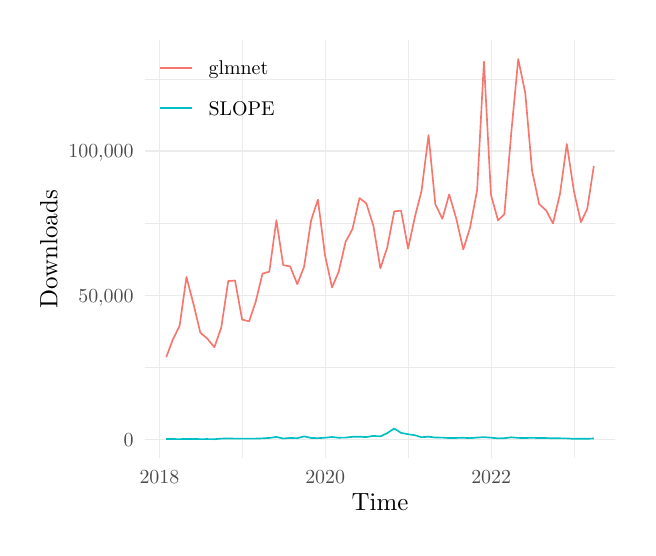
\begin{tikzpicture}[x=1pt,y=1pt]
\definecolor{fillColor}{RGB}{255,255,255}
\path[use as bounding box,fill=fillColor,fill opacity=0.00] (0,0) rectangle (216.81,180.67);
\begin{scope}
\path[clip] ( 42.34, 25.11) rectangle (212.31,176.17);
\definecolor{drawColor}{gray}{0.92}

\path[draw=drawColor,line width= 0.2pt,line join=round] ( 42.34, 57.90) --
	(212.31, 57.90);

\path[draw=drawColor,line width= 0.2pt,line join=round] ( 42.34,110.01) --
	(212.31,110.01);

\path[draw=drawColor,line width= 0.2pt,line join=round] ( 42.34,162.12) --
	(212.31,162.12);

\path[draw=drawColor,line width= 0.2pt,line join=round] ( 77.56, 25.11) --
	( 77.56,176.17);

\path[draw=drawColor,line width= 0.2pt,line join=round] (137.50, 25.11) --
	(137.50,176.17);

\path[draw=drawColor,line width= 0.2pt,line join=round] (197.45, 25.11) --
	(197.45,176.17);

\path[draw=drawColor,line width= 0.5pt,line join=round] ( 42.34, 31.84) --
	(212.31, 31.84);

\path[draw=drawColor,line width= 0.5pt,line join=round] ( 42.34, 83.95) --
	(212.31, 83.95);

\path[draw=drawColor,line width= 0.5pt,line join=round] ( 42.34,136.06) --
	(212.31,136.06);

\path[draw=drawColor,line width= 0.5pt,line join=round] ( 47.61, 25.11) --
	( 47.61,176.17);

\path[draw=drawColor,line width= 0.5pt,line join=round] (107.51, 25.11) --
	(107.51,176.17);

\path[draw=drawColor,line width= 0.5pt,line join=round] (167.49, 25.11) --
	(167.49,176.17);
\definecolor{drawColor}{RGB}{248,118,109}

\path[draw=drawColor,line width= 0.6pt,line join=round] ( 50.07, 61.61) --
	( 52.37, 67.76) --
	( 54.91, 72.98) --
	( 57.37, 90.58) --
	( 59.92, 80.79) --
	( 62.38, 70.47) --
	( 64.92, 68.29) --
	( 67.46, 65.18) --
	( 69.93, 72.20) --
	( 72.47, 89.10) --
	( 74.93, 89.32) --
	( 77.48, 75.20) --
	( 80.02, 74.55) --
	( 82.32, 81.39) --
	( 84.86, 91.79) --
	( 87.32, 92.50) --
	( 89.87,111.09) --
	( 92.33, 94.86) --
	( 94.87, 94.39) --
	( 97.42, 87.99) --
	( 99.88, 94.24) --
	(102.42,111.06) --
	(104.88,118.49) --
	(107.43, 98.50) --
	(109.97, 86.80) --
	(112.35, 92.39) --
	(114.89,103.34) --
	(117.36,107.86) --
	(119.90,119.09) --
	(122.36,117.18) --
	(124.91,109.16) --
	(127.45, 93.71) --
	(129.91,101.18) --
	(132.45,114.27) --
	(134.92,114.57) --
	(137.46,100.86) --
	(140.00,112.66) --
	(142.30,121.57) --
	(144.85,141.85) --
	(147.31,116.82) --
	(149.85,111.61) --
	(152.31,120.44) --
	(154.86,111.69) --
	(157.40,100.53) --
	(159.86,108.46) --
	(162.41,122.01) --
	(164.87,168.39) --
	(167.41,120.22) --
	(169.96,111.06) --
	(172.25,113.25) --
	(174.80,143.32) --
	(177.26,169.31) --
	(179.80,157.08) --
	(182.26,128.99) --
	(184.81,116.96) --
	(187.35,114.60) --
	(189.81,109.94) --
	(192.36,120.66) --
	(194.82,138.64) --
	(197.36,121.67) --
	(199.91,110.36) --
	(202.20,115.18) --
	(204.58,130.72);
\definecolor{drawColor}{RGB}{0,191,196}

\path[draw=drawColor,line width= 0.6pt,line join=round] ( 50.07, 32.03) --
	( 52.37, 32.02) --
	( 54.91, 31.99) --
	( 57.37, 32.06) --
	( 59.92, 32.03) --
	( 62.38, 32.00) --
	( 64.92, 32.01) --
	( 67.46, 31.97) --
	( 69.93, 32.17) --
	( 72.47, 32.25) --
	( 74.93, 32.16) --
	( 77.48, 32.16) --
	( 80.02, 32.18) --
	( 82.32, 32.18) --
	( 84.86, 32.27) --
	( 87.32, 32.42) --
	( 89.87, 32.78) --
	( 92.33, 32.22) --
	( 94.87, 32.42) --
	( 97.42, 32.32) --
	( 99.88, 32.99) --
	(102.42, 32.42) --
	(104.88, 32.34) --
	(107.43, 32.50) --
	(109.97, 32.76) --
	(112.35, 32.50) --
	(114.89, 32.55) --
	(117.36, 32.82) --
	(119.90, 32.87) --
	(122.36, 32.72) --
	(124.91, 33.17) --
	(127.45, 32.98) --
	(129.91, 34.15) --
	(132.45, 35.84) --
	(134.92, 34.25) --
	(137.46, 33.76) --
	(140.00, 33.38) --
	(142.30, 32.68) --
	(144.85, 32.88) --
	(147.31, 32.56) --
	(149.85, 32.54) --
	(152.31, 32.37) --
	(154.86, 32.42) --
	(157.40, 32.47) --
	(159.86, 32.35) --
	(162.41, 32.56) --
	(164.87, 32.70) --
	(167.41, 32.52) --
	(169.96, 32.26) --
	(172.25, 32.33) --
	(174.80, 32.65) --
	(177.26, 32.43) --
	(179.80, 32.41) --
	(182.26, 32.45) --
	(184.81, 32.40) --
	(187.35, 32.37) --
	(189.81, 32.30) --
	(192.36, 32.28) --
	(194.82, 32.26) --
	(197.36, 32.09) --
	(199.91, 32.15) --
	(202.20, 32.12) --
	(204.58, 32.21);
\end{scope}
\begin{scope}
\path[clip] (  0.00,  0.00) rectangle (216.81,180.67);
\definecolor{drawColor}{gray}{0.30}

\node[text=drawColor,anchor=base east,inner sep=0pt, outer sep=0pt, scale=  0.72] at ( 38.29, 29.36) {0};

\node[text=drawColor,anchor=base east,inner sep=0pt, outer sep=0pt, scale=  0.72] at ( 38.29, 81.47) {50,000};

\node[text=drawColor,anchor=base east,inner sep=0pt, outer sep=0pt, scale=  0.72] at ( 38.29,133.58) {100,000};
\end{scope}
\begin{scope}
\path[clip] (  0.00,  0.00) rectangle (216.81,180.67);
\definecolor{drawColor}{gray}{0.30}

\node[text=drawColor,anchor=base,inner sep=0pt, outer sep=0pt, scale=  0.72] at ( 47.61, 16.10) {2018};

\node[text=drawColor,anchor=base,inner sep=0pt, outer sep=0pt, scale=  0.72] at (107.51, 16.10) {2020};

\node[text=drawColor,anchor=base,inner sep=0pt, outer sep=0pt, scale=  0.72] at (167.49, 16.10) {2022};
\end{scope}
\begin{scope}
\path[clip] (  0.00,  0.00) rectangle (216.81,180.67);
\definecolor{drawColor}{RGB}{0,0,0}

\node[text=drawColor,anchor=base,inner sep=0pt, outer sep=0pt, scale=  0.90] at (127.33,  6.25) {Time};
\end{scope}
\begin{scope}
\path[clip] (  0.00,  0.00) rectangle (216.81,180.67);
\definecolor{drawColor}{RGB}{0,0,0}

\node[text=drawColor,rotate= 90.00,anchor=base,inner sep=0pt, outer sep=0pt, scale=  0.90] at ( 10.70,100.64) {Downloads};
\end{scope}
\begin{scope}
\path[clip] (  0.00,  0.00) rectangle (216.81,180.67);
\definecolor{drawColor}{RGB}{248,118,109}

\path[draw=drawColor,line width= 0.6pt,line join=round] ( 47.86,166.05) -- ( 59.42,166.05);
\end{scope}
\begin{scope}
\path[clip] (  0.00,  0.00) rectangle (216.81,180.67);
\definecolor{drawColor}{RGB}{0,191,196}

\path[draw=drawColor,line width= 0.6pt,line join=round] ( 47.86,151.59) -- ( 59.42,151.59);
\end{scope}
\begin{scope}
\path[clip] (  0.00,  0.00) rectangle (216.81,180.67);
\definecolor{drawColor}{RGB}{0,0,0}

\node[text=drawColor,anchor=base west,inner sep=0pt, outer sep=0pt, scale=  0.72] at ( 65.37,163.57) {glmnet};
\end{scope}
\begin{scope}
\path[clip] (  0.00,  0.00) rectangle (216.81,180.67);
\definecolor{drawColor}{RGB}{0,0,0}

\node[text=drawColor,anchor=base west,inner sep=0pt, outer sep=0pt, scale=  0.72] at ( 65.37,149.11) {SLOPE};
\end{scope}
\end{tikzpicture}
